\documentclass{article}
\usepackage[utf8]{inputenc}
\usepackage{xurl}
\usepackage[czech]{babel}
\usepackage{csquotes}
\usepackage{graphicx}
\usepackage{svg}

\MakeOuterQuote{"}

\title{Kontrola typové koherence kontstrukcí Transparentní intenzionální logiky}
\author{Filip Peterek}
\date{9. červen 2022}

\begin{document}

\maketitle

\section{Cíl práce}

Cílem práce bylo vytvoření programu umožňujícího kontrolu typové koherence konstrukcí Transparentní
intenzionální logiky. Program měl na svém vstupu příjímat konstrukce, na svém výstupu měl
vrátit seznam případných chyb, a graficky znázornit průběh typové kontroly za využití grafu.

Program je psán v programovacím jazyce Kotlin, jako build systém byl zvolen Gradle.

V současném stavu je program CLI aplikací. Při spouštění lze programu předat libovolný počet souborů
jako CLI argumenty. Tyto soubory jsou poté postupně zpracovány programem. Program všechen svůj
výstup vytvoří ve složce, ze které byl spuštěn. Pro každý vstupní soubor jsou vytvořeny nanejvýš
dva výstupní soubory, textový výstup ve formátu JSON~\cite{json-src} popisující vstupní TIL-Script program, a graf
typové kontroly ve formátu SVG~\cite{svg-src}. Název výstupního souboru je definován jako název
vstupního souboru, za něž je pouze dodána přípona odpovídající danému formátu. Soubory nemusí být
vytvořeny, pokud je vytvořit nelze (např. z důvodu chyby ve vstupním programu). Žádné přepínače
poté program neočekává.

\section{Transparentní intenzionální logika}

Transparentní intenzionální logika~\cite{til-duzi} (dále také pouze TIL) je logický systém sloužící
k analýze přirozeného jazyka. TIL vychází z typovaného lambda kalkulu, a využívá rigorózně definovaný
typový systém za účelem zabránění velké škále chyb. Mezi chyby, které lze typovým systémem zachytit,
patří například primitivnější chyby, jako je špatné pořadí argumentů (rovnice počítá Karla), ale také
chybná změna supozice způsobená inkorektní analýzou (funkce očekává úřad, avšak na vstupu dostane
individuum). Kontrolu typové koherence však lze provádět strojově. Tato práce se zabývá automatizací
typové kontroly, jež je užitečná převážně v případě, kdy analyzujeme složité TIL konstrukce a manuální
typová kontrola by tedy byla náchylná k chybě.

\subsection{TIL-Script}

TIL-Script~\cite{til-script} je funkcionální programovací jazyk sloužící k práci s TIL konstrukcemi.
Syntax TIL-Scriptu vychází z notace TIL, kterou je však upravena pro~potřeby počítačového zápisu -- zatímco
TIL ve své notaci hojně využívá řecké abecedy nebo horních i dolních indexů, TIL-Script byl vytvářen
tak, aby byl jednoduše zapisovatelný i na běžné klávesnici. Z toho důvodu byl také TIL-Script zvolen
jako notace využívaná v této práci.

\section{Implementace}

\subsection{Parser jazyka TIL-Script}

Parser byl vygenerován za využití generátoru parserů Antlr~\cite{antlr-src}. Díky volby již existujícího
jazyka jako notace programu stačilo gramatiku jazyka TIL-Script upravit do formátu zpracovatelného
Antlrem. Jelikož program pro kontrolu typové koherence využívá build systém Gradle, je parser automaticky
vygenerován během kompilace, je-li to potřeba. Výstup vygenerovaného parseru je poté převeden na vlastní
reprezentaci, která je méně generická a umožňuje ergonomičtější programatickou práci s abstraktním
syntaktickým stromem TIL-Script programu.

Ke kontrole syntaktických chyb je využita kontrola zabudovaná do nástroje Antlr. Nad rámec automatického
reportování zabudovaného v Antlru je implementován pouze vylepšený indikátor pozice chyby přímo
ve strojovém kódu, a kromě číselné pozice chyby je vypsán také samotný chybný řádek s graficky vyznačenou
chybou.

\subsection{Kontrola existence symbolů}

Aby bylo možné provést typovou kontrolu, je třeba znát typy všech symbolů, které se ve vstupní konstrukci
nacházejí. Proto tvorbu abstraktního syntaktického stromu následuje právě kontrola, zda jsou všechny
symboly definovány. Symbol může být definován jako literál (např. Karel, Vysoká škola báňská), funkce,
proměnná libovolného typu, nebo jako typový alias (ekvivalent např. \texttt{typedef} známého z jazyků
C a C++). Typové aliasy, literály a funkce lze definovat pouze pomocí samostatné TIL-Script definice.
Proměnné lze definovat pomocí globální definice definující volnou proměnnou, nebo jako $\lambda$-vázanou
proměnnou v konstrukci uzávěru. Symbol musí být definován před jeho prvním použitím.

Proměnné vázané trivializací také musí být definované. Ačkoliv proměnné vázané trivializací nejsou
konstituenty, neboť trivializace konstruuje konstrukci proměnné, tedy typ $*_{n}$, program provádí typovou
kontrolu všech podkonstrukcí.

V případě, že se vstupní program odkazuje na alespoň jeden nedefinovaný symbol, je běh programu ukončen a
na~standardní výstup jsou vypsány všechny využívané, avšak nedefinované symboly. K typové kontrole nedojde,
neboť ji nejde provést.

Program automatickou dedukci typů symbolů nepodporuje.

\subsection{Kontrola typové koherence}

Kontrola typové koherence vyžaduje průchod stromem a proto je, přirozeně, implementována rekurzivně. Při
kontrole každé konstrukce jsou zkontrolovány nejprve její podkonstrukce (všechny podkonstrukce, nejen
konstituenty). Podkonstrukce jsou zkontrolovány, zda jsou typově koherentní, a je jim přirazen datový
typ, který konstruují. Teprve poté je zkontrolována původní konstrukce. Atomickým konstrukcím, tedy
proměnným, literálům a funkcím, je jejich typ přirazen rovnou.

V kompozici, tedy při aplikaci funkce, je třeba zkontrolovat, že je funkce aplikována na správný počet
argumentů, a že všechny typy argumentů odpovídají typům dle signatury funkce. V opačném případě
samozřejmě typová kontrola selhává a na~standardní výstup je vypsána chyba.

Selže-li typová kontrola v některé z podkonstrukcí, typová kontrola konstrukce samotné selhává také,
neboť ji nelze provést. V takovém případě však není vypisována žádná chyba, neboť program v současné
verzi nedokáže určit, zda by k chybě došlo. Typ konstruovaný konstrukcí je označen za neznámý. Jelikož
kontrola existence symbolů byla provedena již v předchozím kroku, lze v tomto kroku přítomnost neznámého
typu interpretovat právě jako selhání typové kontroly.

Datové typy jsou konstrukcím přiřazovány teprve při úspěšném dokončení typové kontroly pro danou konstrukci.
Důvodem této implementace je existence typově polymorfních funkcí, u kterých nemusí být předem jednoznačně
určen konstruovaný typ.

Při typové kontrole je nutné brát v potaz vázání proměnných. Proto je pro každou trivializaci konstrukce, jež
není literál nebo funkce, a pro každý uzávěr konstruován nový kontext. Kontext trivializace je nezávislý na
kontextu nadkonstrukce, odkazuje se pouze na globální kontext, jež obsahuje informace o~volných proměnných
a funkcích. Kontext uzávěru se na kontext nadkonstrukce odkazuje, umožňuje však definovat $\lambda$-vázané proměnné,
jež zastíní proměnné z~rodičovských kontextů. Při nalezení symbolu jsou poté kontexty prohledávány rekurzivně,
od nejbližšího kontextu až po kontext globální, a je hledán typ konstruovaný symbolem. Globální kontext je
samozřejmě nezávislý na kontextech uzávěrů a trivializací. Lze jej modifikovat pouze globální definicí.

Dále je důležité vyřešit porovnávání uživatelem definovaných typových aliasů a typů jimi reprezentovanými.
Při porovnávání typů jsou vždy všechny aliasy rekurzivně expandovány, dokud se datový typ neskládá pouze
z typů zabudovaných přímo do jazyka TIL-Script. Teprve takto plně expandované typy se mezi sebou porovnávají.
Tento způsob porovnávání uživatelem definovaných typů byl zvolen zejména proto, že TIL-Script neumožňuje
definici nového typu např. definicí struktury složené z více hodnot již existujících typů, ale pouze definici
nového názvu pro již existující typ.

Dvojité provedení není kontrolováno, neboť pro něj obecně není možné korektně určit konstruovaný typ.

\subsection{Rozpoznání kontextu}

Po dokončení typové kontroly je provedeno také rozpoznání kontextu. V tomto kroku se pouze rozhoduje, zda
se jednotlivé konstrukce nachází ve výskytu hyperintenzionálním, intenzionálním, či extenzionálním. Informace
o výskytu se nachází pouze v textovém výstupu programu, graficky momentálně výskyt nijak znázorňován není.

Implementace je opět rekurzivní. Program rekurzivně vyhodnocuje výskyt vstupní konstrukce a poté všech jejich
podkonstrukcí. Zároveň vždy uchovává informaci o nejvyšším nadřazeném kontextu, neboť je při rozpoznávání
kontextu nutné kontrolovat, zda se konstrukce nenachází ve vyšším nadřazeném kontextu. V takovém případě se
totiž výskyt konstrukce rovná výskytu nadřazenému.

\section{Výstup programu}

\subsection{Grafický výstup}

Jako formát grafického výstupu byl zvolen vektorový grafický formát SVG. Opodstatněními volby tohoto formátu
jsou jeho jednoduchost a textová nátura, jež umožňují jednoduché generování SVG obrázků, rozšířenost formátu,
ale také vektorová charakteristika, díky které lze SVG obrázky libovolně škálovat bez~ztráty kvality~\cite{svg-src}.

Grafický výstup znázorňuje pouze průběh typové kontroly. Chyby či výskyty konstrukcí znázorňovány nejsou.

V grafu je znázorněna nejen původní konstrukce, ale hlavně také typy konstruované konstrukcí samotnou i jejími
podkonstrukcemi. Pro textový výpis konstrukcí a typů byl zvolen neproporcionální font. Tato volba umožňuje přesně
spočítat pozici každého znaku, protože všechny znaky mají nutně stejnou šířku. Tento fakt je využit při definici
čar spojujících konstrukce a typy. Jelikož názvy typů můžou být v jazyce TIL-Script relativně dlouhé, musí být
typy, ale konstrukce tyto typy konstruující, odsazeny, aby nedošlo k překrývání textu. Ukázku grafu
typové kontroly lze vidět na obrázku~\ref{fig:graph}.

\begin{figure}
    \centering
    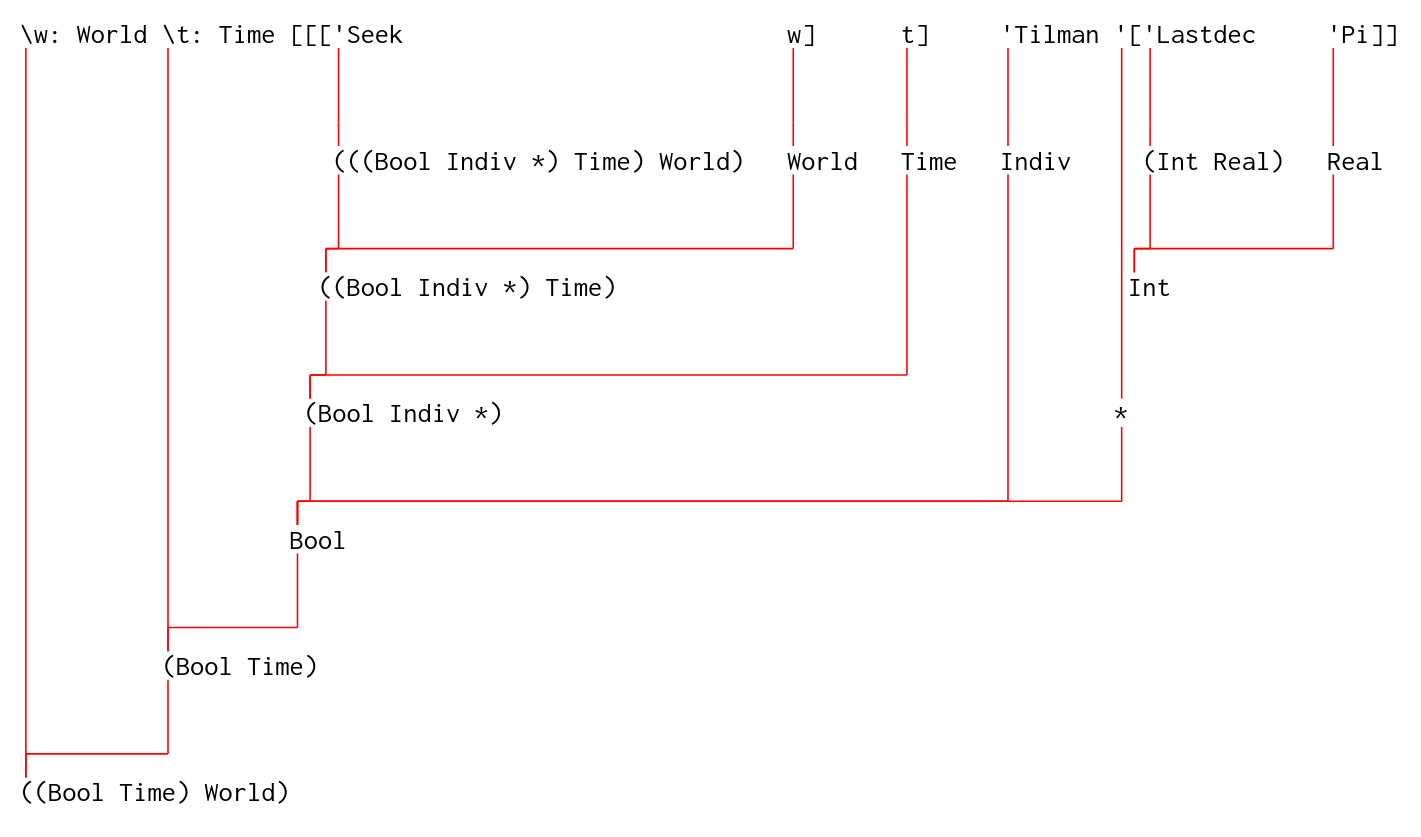
\includegraphics[width=0.9\textwidth]{graph.png}
    \caption{Ukázka grafu typové kontroly}\label{fig:graph}
\end{figure}

Algoritmus tvorby grafu typové kontroly byl psán ručně, nejsou použity žádné knihovny třetí strany.

\subsection{Textový výstup}

\subsubsection{Standardní výstup}

Jelikož se jedná o CLI aplikaci, program k interakci s uživatelem využívá standardní výstup. Na~standardní
výstup program vypisuje chyby ve vstupních souborech -- o jakou chybu se jedná, na jaké pozici se chyba nachází,
a také úryvek relevantního kódu se znázorněnou chybou.

\subsubsection{JSON výstup}

Výstup ve formátu JSON je zapsán do souboru. JSON výstup obsahuje informace o obsahu souboru -- jaké konstrukce
se v něm nachází, podkonstrukce jednotlivých konstrukcí, typ konstruovaný každou konstrukcí, typ konstrukce,
ale také výskyt konstrukce. Z JSON souboru lze plně zrekonstruovat vstupní soubor, s výjimkou formátování textu.

Důvodem volby formátu JSON byly převážně plány rozšířit v budoucnu program o webovou aplikaci nebo jazykový server.
Protokol LSP dle svého standardu ke komunikaci využívá formát JSON. Ve~webových aplikacích je poté formát JSON
víceméně standard díky všudypřítomnosti jazyka Javascript. Formát JSON je samozřejmě pro aktuální aplikaci
velmi dobře využitelný, neboť slouží ke kódování stromových struktur~\cite{json-src}, které jsou pro reprezentaci konstrukcí
složených z podkonstrukcí velmi praktické.

\section{Závěr}

Zadáním projektu bylo implementovat typovou kontrolu a znázornit ji pomocí grafu. Zadání bylo splněno. Program
je dále možné rozšířit například o implementaci protokolu LSP~\cite{lsp-src}, což by umožnilo ergonomičtější tvorbu a editaci
TIL-Script programů v editorech implementujících tento protokol. Alternativně by bylo možné vytvořit interaktivní
webovou službu umožňující provádět typovou kontrolu v prohlížeči.


\begin{thebibliography}{50}

\bibitem{til-duzi}
Duží, M., Materna, P.: \textit{TIL jako procedurální logika} \\
Marie Duží, Pavel Materna, 2012

\bibitem{til-script}
Ciprich, N., Duží, M., Košinár, M.: \textit{TIL-Script: Functional Programming Based on
Transparent Intensional Logic} \\
In: \textit{RASLAN 2007}, Sojka, P., Horák, A., (Eds.), Masaryk University Brno, 2007, pp. 37–42.

\bibitem{antlr-src}
Parr, T.: \textit{ANTLR v4} [online, cit. 2022-06-09] \\
Dostupné z: \url{https://www.antlr.org} \\
Terence Parr

\bibitem{svg-src}
W3C: \textit{Scalable Vector Graphics (SVG) 2} [online, cit. 2022-06-09] \\
Dostupné z: \url{https://www.w3.org/TR/SVG2/} \\
World Wide Web Consorcium

\bibitem{json-src}
ECMA: \textit{JSON} [online, cit. 2022-06-09] \\
Dostupné z: \url{www.json.org} \\
ECMA

\bibitem{lsp-src}
Microsoft: \textit{Language Server Protocol} [online, cit. 2022-06-09] \\
Dostupné z: \url{https://microsoft.github.io/language-server-protocol/} \\
Microsoft

\end{thebibliography}

\end{document}

